%        File: Intro.tex
%     Created: Sun Mar 02 03:00 PM 2014 P
% Last Change: Sun Mar 02 03:00 PM 2014 P
%
\documentclass[letterpaper,12pt]{report}
\usepackage[sorting=none,backend=bibtex]{biblatex}
\usepackage{fullpage}
\usepackage{hyperref}
\hypersetup{colorlinks=true,urlcolor=blue}
\usepackage[all]{hypcap}
\usepackage{amsmath}
\usepackage{graphicx}
\usepackage[font=small,labelfont=bf]{caption}
%\usepackage[doublespacing]{setspace}
%\usepackage[onehalfspacing]{setspace}
\addbibresource{CapstoneCitations.bib}

\pagestyle{plain}

\title{Humanoid Robotic Subsystems}
\date{April 14, 2014}
\author{Wenbo Wang \\University of California, Berkeley}

\begin{document}

\begin{titlepage}
\begin{center}

% Upper part of the page. The '~' is needed because \\
% only works if a paragraph has started.

    \textsc{\large University of California, Berkeley College of Engineering}\\[0.5cm]
    \textsc{\Large MASTER OF ENGINEERING - SPRING 2014}\\[1.5cm]

    \textsc{\large Electrical Engineering and Computer Sciences}\\[0.5cm]
    \textsc{\LARGE Humanoid Robotics Subsystems}\\[0.5cm] 
    \textsc{\LARGE Wenbo Wang}\\[1.5cm]

\end{center}

\begin{flushleft}
{
    This Masters Project Paper fulfills the Master of Engineering degree
    requirement\\[0.5cm]
    Approved by:\\[0.5cm]
    1.  Capstone Project Advisor: \\[0.5cm]
    Signature: \underline{\hspace{7cm}} Date \underline{\hspace{3cm}}\\[0.5cm]
    Print Name: Donald Wroblewski\\
    Department: Fung Institute\\[1.5cm]

    2. Faculty Committee Member \#2: \\[0.5cm]
    Signature: \underline{\hspace{7cm}} Date \underline{\hspace{3cm}}\\[0.5cm]
    Print Name: Ruzena Bajcsy\\
    Department: Electrical Engineering and ComputerSciences\\
}
\end{flushleft}

\end{titlepage}


\begin{abstract}
There is a growing need for robots in many different sectors of industry. As
demand increases and technology improves there will be a great demand for robots
that can better integrate into the workplace and the home. Humanoid robotics are
a potential technology that can bridge this gap. Our sponsor, Bay Area IP LLC,
is exploring new Intellectual Property potential in this exciting field. We have
designed and prototyped many humanoid robot components that can be used as a
platform for exploring potential technologies as wells as serve as sources of
new IP. This report describes the prototype robot leg and embedded software
system for the robot platform, as well as summarizing the other subsystems
worked on by the team.
\end{abstract}

\section{Introduction}
\paragraph{}Robots are being widely adopted by in many industries, and there is
a growing need for humanoid robotics. Humanoid robotic components can have many
applications such as manufacturing and prosthetics. A key component of our
project, the mechanical design of a humanoid robotic hand can be applied to both
manufacturing and prosthetics. Currently humanoid robots and robot subsystems
are not in wide use, so it is a good target for our sponsor, Bay Area IP, which
is looking do develop intellectual property that they could license to others.

\paragraph{}There are many technical challenges that come with trying to
reproduce the human form. The human body is very complex and there are many
different components that need to interact and function correctly. The human
hand has 27 degrees of freedom, and it is very difficult to reproduce that
complexity \cite{ElKoura2003}. However, modern manufacturing techniques such as
3D printing can get us closer to reproducing that complexity. Reproducing human
capabilities through software is also a great challenges. It is difficult to
design and implement complex control systems capable of mimicking the human
body. New computer hardware is allowing us to create more complex robots capable
of performing human like tasks.

\paragraph{}The subsystems we designed were the arms, hands, legs, feet, and
vision systems.  We designed the mechanical structure of these components and
the software for controlling the different parts. For the hands we did CAD
design of the hand structure. We also performed tests on using shape memory
alloy(SMA) to actuate components of in the fingers. Simple prototypes of the
arms and legs were constructed using off-the-shelf components to provide testing
platforms for the software. The control software was simulated in MATLAB and
then implemented in C++ on a microcontroller. The computer vision system was
implemented on an AMD APU, and utilized a novel laser system to augment the
computer vision algorithms.

\paragraph{}I was responsible for the construction of the mechanical arm, leg,
and the programming of the microcontroller. We implemented a simple control
algorithm for robot walking. This report will describe the materials and methods
used to construct the arms, and legs, as well as the programming of the
microcontroller for basic control of the robot. I will also give an overview of
the other components of the project.

\section{Literature Review}
\subsection{Computer Vision}
\paragraph{}Object detection has been well studied in a variety of applications.
Many machine learning algorithms are utilized for object detection such as
Support Vector Machines or Convolutional Neural
Networks\cite{Barbu2012},\cite{krizhevsky2012imagenet}. Many of the object
detection algorithms utilize Histogram of Oriented Gradient(HOG) features, which
are based on taking a gradient over the image and generating histograms of
gradient angles and magnitudes using overlapping sections of the
image\cite{Dalal2005}. 

\paragraph{}Complex object detection algorithms can be very resource intensive,
as they often need to scan the image multiple times at different resolutions to
find all the objects\cite{Felzenszwalb2013}. This can be a very expensive
process on an embedded system such as the robot. In a cluttered space it can be
very difficult to detect robots correctly in real time. On a robotic system
there usually exist other sensors that can supplement the visual information to
help ease this process. Utilization of depth sensors can help process the visual
information more easily\cite{Gould2008}.

\paragraph{}Computer vision techniques could have many applications for
manufacturing robots. As manufacturing robotics advance, they will need more
accuracy and intelligence to accomplish their tasks, and vision is a good tool
for accomplishing this. Already there are manufacturing robots utilizing vision
for tasks such as part recognition and sorting\cite{SIRfuture}.

\subsection{Robotic Hand}
\paragraph{}There are many different companies and research groups constructing
robotic hands for many different applications. There are hands designed to be
prosthetics, as well as hands designed to be integrated into robotic systems.
One of the most complex is the UB Hand IV, this hand is nearly the same as a
human hand in terms of capabilities. However, the hand is very heavy and very
power hungry, so it is not very suitable for most
applications\cite{Melchiorri2013}. However, most light weight hands are lacking
in complexity and function. The this recently developed lightweight hand only
has five degrees of freedom\cite{takaki2011high}. To develop a hand that is both
light weight, small, and fully functional will require new design techniques. 

\subsection{Shape Memory Alloy}
\paragraph{}We want to leverage some modern technology to make a robotic hand
that is smaller and light weight. One potential tool is Shape Memory Alloy
(SMA), a type of material that can expand or contract when
heated\cite{Schetky1982}. Many metallic alloys exhibit the shape memory
effect\cite{Wayman1993}. These alloys can be deformed at a lower temperature,
when heated, they will return to their original shape. We can use this do
accomplish actuation using a small form device heated through electrical
current\cite{Ikuta1990}. This actuation can be used in the fingers of the hand
, where space is very limited.

\subsection{Robot Leg}
\paragraph{}A popular control method for robot locomotion is Central Pattern
Generators (CPG). Central pattern generators are neural networks that generate
periodic control signals in the body. This control can be generated in the
absence of feedback signals. The human body utilizes this
system for many different rythmic motor functions that the body needs to
perform\cite{cpggeneral}. 

\paragraph{}Central pattern generator can also be adapted to the locomotion of
robots. CPG can be used to control locomotion of bipedal robots, as well as
hexapods and octopods. Using coupled oscillators one can design a control system
for bipedal robots. CPG are well suited for feedback control of bipedal
locomotion. Properly implemented CPG also allow for higher level control of the
walking without needing to worry about exact servo outputs. However CPGs are not
well understood and difficult to design properly\cite{Ijspeert2008}.

\subsection{Robot Arm}
\paragraph{}For the controls of our robot arm we will be implementing Fuzzy
Logic control systems. These control systems can handle nonlinearities well they
are well studied for control of robotic systems such as arms\cite{Scharf1985}.
Fuzzy logic controllers can also be used to control balance of the robotic legs,
treating the legs as an inverted pendulum\cite{hwang1992stability}.

\paragraph{}Rather than using complex models, a fuzzy logic controller relies on
empirical rules, this makes the controller computationally cheap and well suited
for embedded applications. A fuzzy logic controller has three main components: a
fuzzifier, a rule base, and an defuzzifier. In the fuzzifier, analog inputs are
fuzzified into fuzzy logic values between 0 and 1. The fuzzy values are put into
the rule base to determine a set of fuzzy outputs, and then the defuzzifier
combines the outputs into an analog output\cite{Mailah2000}.


\section{Materials and Methods}
\subsection{Materials}
\paragraph{PIC32MX795F512L:}A 32 bit micro-controller for performing the control
algorithms of the robot. The PIC32MX795F512L comes from SparkFun electronics as
part of the UBW32 board, which comes preloaded with a bootloader for programming
the board. See figure \ref{ubw32fig} for an image of the UBW32 board. The
PIC32MX795F512L is programmed in C/C++. To make the device easier to use, we
loaded an avrdude bootloader onto the device to use the MPIDE software. The
MPIDE framework allows us to use Arduino libraries on the PIC32MX795F512L which
helps to accelerate development of basic I/O software for the
board\cite{pic32data}.

\begin{figure}
  \centering
    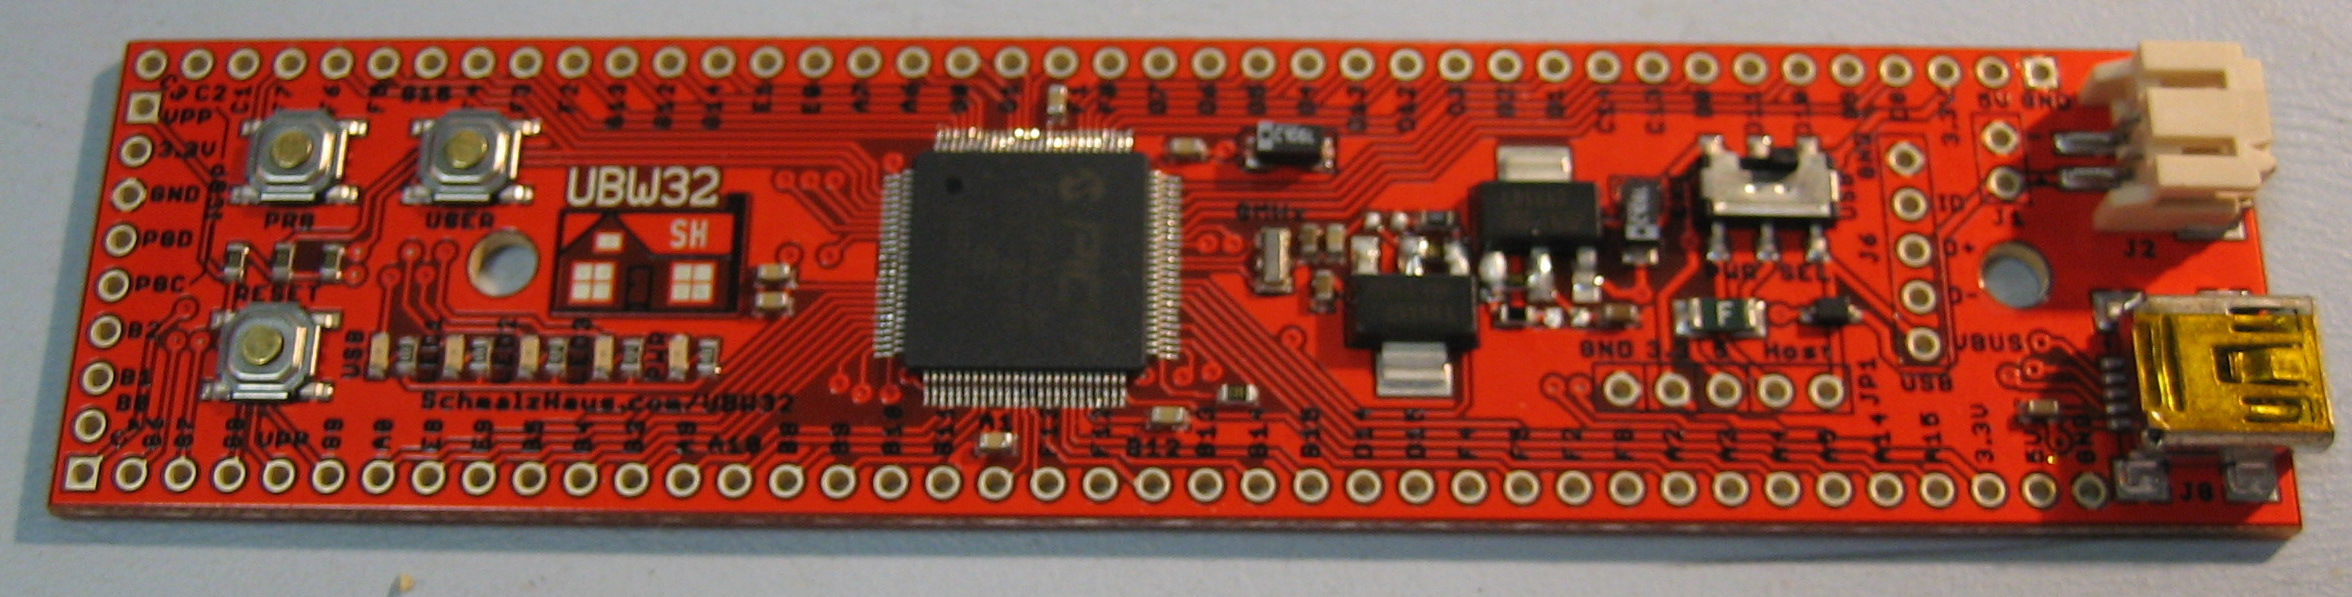
\includegraphics[width=0.75\textwidth]{figures/UBW32_v24_SparkFun.JPG}
  \caption{UBW32 board from SparkFun electronics}
  \label{ubw32fig}
\end{figure}

\paragraph{PICKIT3:}A hardware programmer for the PIC32MX795F512L
microprocessor. See figure \ref{pickit3fig}. The pickit3 and program and debug
the PIC32 micro-controller.  Used to download code onto the UBW32. Useful for
installing new bootloaders onto the UBW32 and for restoring broken
firmware\cite{pickitdata}.

\begin{figure}
  \centering
    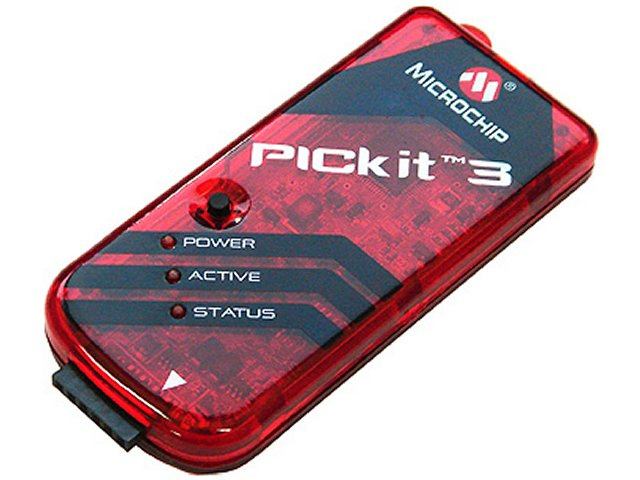
\includegraphics[width=0.3\textwidth]{figures/pickit3.jpg}
  \caption{PICkit 3 In-Circuit Debugger from Microchip}
  \label{pickit3fig}
\end{figure}

\paragraph{MPU6050:}A gyro and accelerometer for obtaining information about the
kinematics of the arm and the leg. See figure \ref{mpufig}. Uses I2C connection
to the PIC32MX795F512L for communication\cite{mpu6050data}.

\begin{figure}
  \centering
    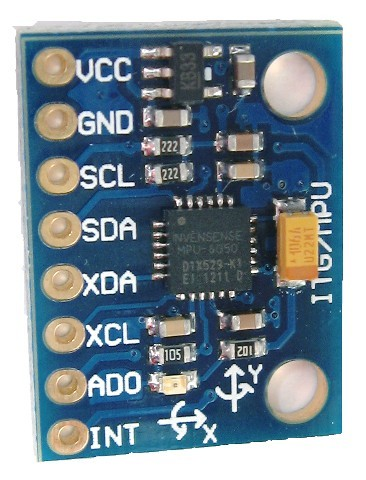
\includegraphics[width=0.2\textwidth]{figures/mpu-6050.jpg}
  \caption{MPU-6050 Triple axis accelerometer and gyro}
  \label{mpufig}
\end{figure}

\paragraph{HSR-5498SG:}Servos from Hitec. Utilized to control arm and leg
joints. See figure \ref{hsrfig}. The servos require 6-7 Volts. Each servo
requires at least 200mA when running without load, and over 1A when stalled.
The actuation of the arm is accomplished by mini-motors rather than
servos\cite{sscdata}.

\begin{figure}
  \centering
    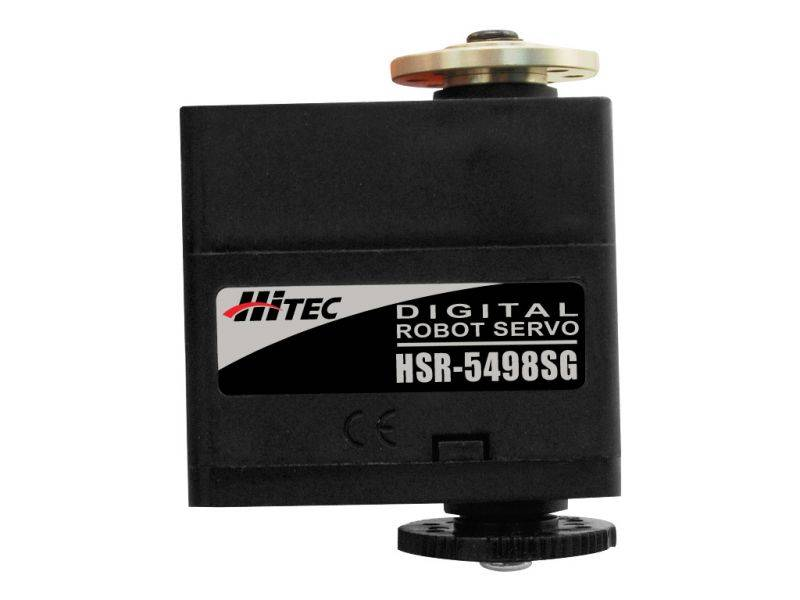
\includegraphics[width=0.4\textwidth]{figures/191_1_HSR-5498SG_HMI_Premium_Robot_Servo-1.jpg}
  \caption{HSR-5498SG servo from Hitech}
  \label{hsrfig}
\end{figure}

\paragraph{SSC-32:}Servo controller from Lynx motion. The on-board controller is
an Atmega168-20PU. See figure \ref{sscfig}. The SSC-32 is controlled using
serial signals from another microprocessor or the PC. The control signal is a
simple byte stream. The controller can specify pin number, servo position,
rotation speed, and rotation time. It can power 32 servos
simultaneously\cite{servodata}.

\begin{figure}
  \centering
    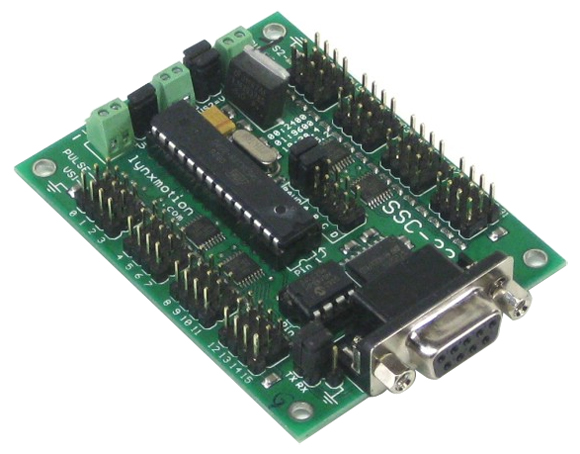
\includegraphics[width=0.4\textwidth]{figures/lynxmotion-ssc-32-servo-controller-large.jpg}
  \caption{SSC-32 servo controller from Lynxmotion}
  \label{sscfig}
\end{figure}

\paragraph{VLT100-4002}Power supply for powering the servos. See figure
\ref{vltfig}. 5V output capable of supplying 3A to 12A of current\cite{vltdata}.

\begin{figure}
  \centering
    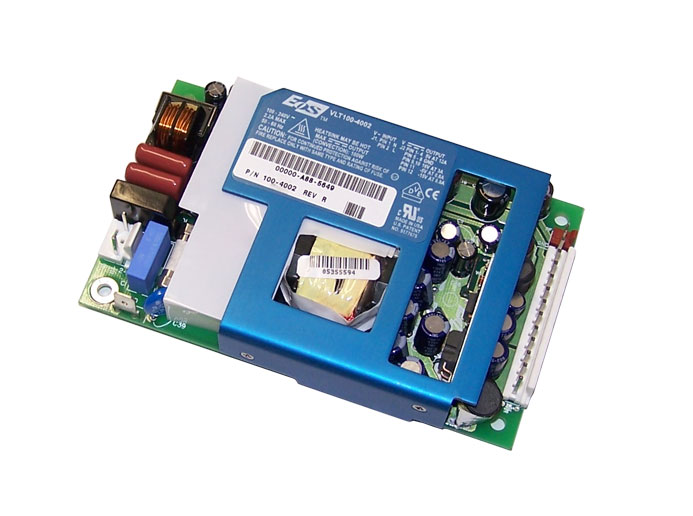
\includegraphics[width=0.4\textwidth]{figures/VLT100-4002.jpg}
  \caption{VLT100-4002 power supply}
  \label{vltfig}
\end{figure}

\paragraph{Yihua 1502DD}Adjustable power supply for servos. See figure
\ref{yihuafig}. 0-15V output and 0-2A output\cite{yihuadata}. 

\begin{figure}
  \centering
    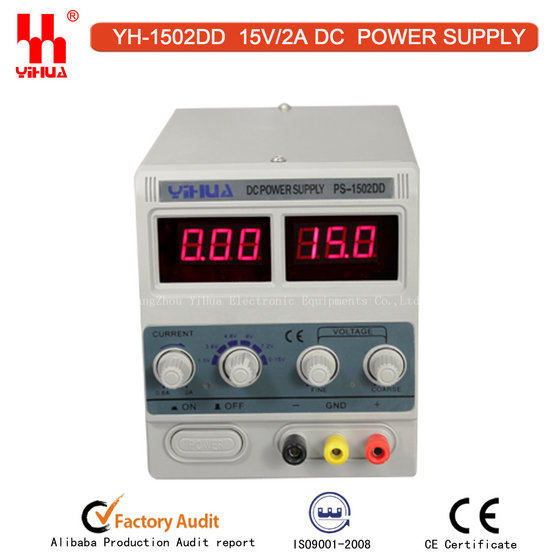
\includegraphics[width=0.4\textwidth]{figures/Power_Supply_YIHUA_1502DD.jpg}
  \caption{Yihua 1502DD DC power supply}
  \label{yihuafig}
\end{figure}

\subsection{Methods}
\subsubsection{Microcontroller Setup}
\paragraph{}To program the PIC32MX795F512L, we used the Multi-Platform
Integrated Development Environment(MPIDE) environment from chipKIT. To use MPIDE
with the program, we had to program the PIC32 with the avrdude bootloader found
here: \url{https://github.com/chipKIT32/PIC32-avrdude-bootloader}. Using the
pickit3, we loaded the new bootloader onto the UBW32 and was able to use MPIDE
to program the board. MPIDE utilizes the Arduino libraries and Arduino style C++
code for programming the board. Through MPIDE, there are a wide variety of
libraries available for performing basic I/O tasks using the PIC32.

\subsubsection{MPU-6050 Setup}
\paragraph{}The MPU-6050 utilizes an I2C connection to the read and write data.
The device readings are stored on a 1024 byte FIFO buffer on the
MPU\cite{mpu6050data}. The MPU can be used to acquire sensory information for
controlling the motions of the legs and the arms. We set up the MPU6050 using
the PIC32 I2C libraries in MPIDE. We utilized the \verb!Wire.h! library to read
and write to the I2C bus of the PIC32\cite{Krodal2013}. There are a total of
five SDA pins on the PIC32MX795F512L, so we can have a minimum of five of these
devices connected to our microcontroller.

\subsubsection{Servo Setup}
\paragraph{}The servos each had a range of 180 degrees. The SSC-32 represents
this as a value between 500 and 2500. Due to the mechanical construction most
joints had a limited range of motion. Most joints had a range of 100 degrees.
The exact ranges were tested and calibrated after the completion other robot
leg. Each servo requires approximately 6V and 200mA to 1A of current depending
on the load\cite{servodata}. For our tests, we used the Yihua DC power supply
which is adjustable up to 15V and supplied up to 2A\cite{yihuadata}.

\subsubsection{Servo Control}
\paragraph{}To control the servos we utilized a SSC-32 servo controller. The
controller has 32 channels for servo control. Each channel can be given a
position, rotation speed, and rotation time. Multiple servo channels can be
controlled simultaneously through a single command The SSC-32 is powered through
a 9V battery. The controls are given in the form of strings, the following is an
example of the commands used for SSC-32.
\begin{verbatim}
#5 P1600 T1000 <cr>
\end{verbatim}
The \#5 defines the channel number which ranges from 0 to 31. The P1600 sets the
position of the servo from 500 to 2500. The T1000 sets the time of rotation in
milliseconds. The carriage return(\verb!<cr>!) signifies the completion of a
command. The following is an example command for simultaneous movement of
servos:
\begin{verbatim}
#5 P1600 #10 P750 T2500 <cr>
\end{verbatim}
In this case all the servos adjust their speed so they arrive at the specified
position in the specified time.

\subsubsection{Walking Algorithm Implementation}
\paragraph{} The walking algorithms were designed by Zhu Ziqi, a fellow team
member. He designed and simulated the algorithms in MATALB and SIMULINK and I
implemented the algorithms in C++ on the PIC32MX795F512L. The servo positions
were determined from a linear combination of sine waves. For our preliminary
walking algorithms we only considered the knee and hip joints. The SSC-32
position control signal requires a integer ranged from 500 to 2500,
corresponding to $180^{\circ}$ of motion\cite{sscdata}. Due to the mechanical
construction of the arm and leg joints, which mimicked human structure, most
joint servos were limited to a range between 1250 and 2500. The output from the
sine waves would be converted to a range in the SSC-32's output and then sent to
the servos. Equations \ref{thetahip} and \ref{thetaknee} show the equations for
calculating the position of each servo as a function of time. The angle of the
hip is a degree relative to the vertical axis of the 3D space, while the angle
of the knee is relative to the axis along the thigh of the robot.
\begin{align}
    \phi_{3}(t)&=a_{13L}sin(b_{13L}t+c_{13L})+a_{23L}sin(b_{23L}t+c_{23L})+a_{33L}sin(b_{33L}t+c_{33L})\nonumber\\
    &+a_{43L}sin(b_{43L}t+c_{43L})+a_{53L}sin(b_{53L}t+c_{53L})+a_{63L}sin(b_{63L}t+c_{63L})\nonumber\\
    &+a_{73L}sin(b_{73L}t+c_{73L})+a_{83L}sin(b_{83L}t+c_{83L}) \label{phi3}\\
    \phi_{4}(t)&=a_{14L}sin(b_{14L}t+c_{14L})+a_{24L}sin(b_{24L}t+c_{24L})+a_{34L}sin(b_{34L}t+c_{34L})\nonumber\\
    &+a_{44L}sin(b_{44L}t+c_{44L})+a_{54L}sin(b_{54L}t+c_{54L})+a_{64L}sin(b_{64L}t+c_{64L})\nonumber\\
    &+a_{74L}sin(b_{74L}t+c_{74L}) \label{phi4}\\
    \theta_{hip}(t)&=\frac{\phi_{3}(t)}{180\pi} \label{thetahip}\\
    \theta_{knee}(t)&=\frac{\theta_{hip}(t)-\phi_{4}(t)}{180\pi} \label{thetaknee}\\
\end{align}
The conversion from angle in degrees to servo position is given by the following
equation.
\begin{align}
    P=\frac{\theta}{180}*2000+500
\end{align}
The positions of the legs are calculated by the PIC32 and sent to the SSC-32
through the Universal Asynchronous Receiver Transmitter(UART) module of the
PIC32. The UART is a serial connection between the PIC32 and the SSC-32. The
calculated results are composed into a string in the form of an SSC-32 command
and sent to the servo controller. 

\section{Discussion}
\subsection{Overall System}
\paragraph{}Currently we have components of a robotic platform prototyped and
designed. The Robotic legs and arm are prototyped and constructed. The hand and
feet have been designed. The basic software and control framework has been
established. The basic I/O and control tasks have been implemented in C++ on the
microcontroller with easy to use APIs that others can use to control the
currently completed robot legs. Overall we are at a good position for the
sponsor to take the foundations we have built and try to implement new different
control algorithms and machine learning algorithms. 

\subsection{Robot Leg}
\paragraph{}The leg was constructed using with six servos on each leg. Three
servos on the hip mimicked the ball and socket configuration of the human hip
joint, which has three degrees of freedom\cite{SiasJr1990}. The three modes of
motion are along the sagittal, frontal, and transverse planes\cite{Fiscell2005}.
The knee has one degree of freedom, and the ankle has two degrees of freedom in
the sagittal and frontal planes. Each leg has six degrees of freedom in total,
this is fine for most gaits on uneven ground, but sudden changes such as steps
would be difficult to manage\cite{SiasJr1990}. More degrees of freedom may be
needed to obtain more human like gait\cite{SiasJr1990}.

\paragraph{}The shins and pelvis were constructed from aluminum U channels. The
thighs where made from aluminum cylinders, and the feet were aluminum plates.
Figure \ref{protolegfig} shows the complete product. The SSC-32 servo controller
was attached to the hip. A wire connects the servo controller to the power
supply and the PIC32 controller. 

\begin{figure}
  \centering
    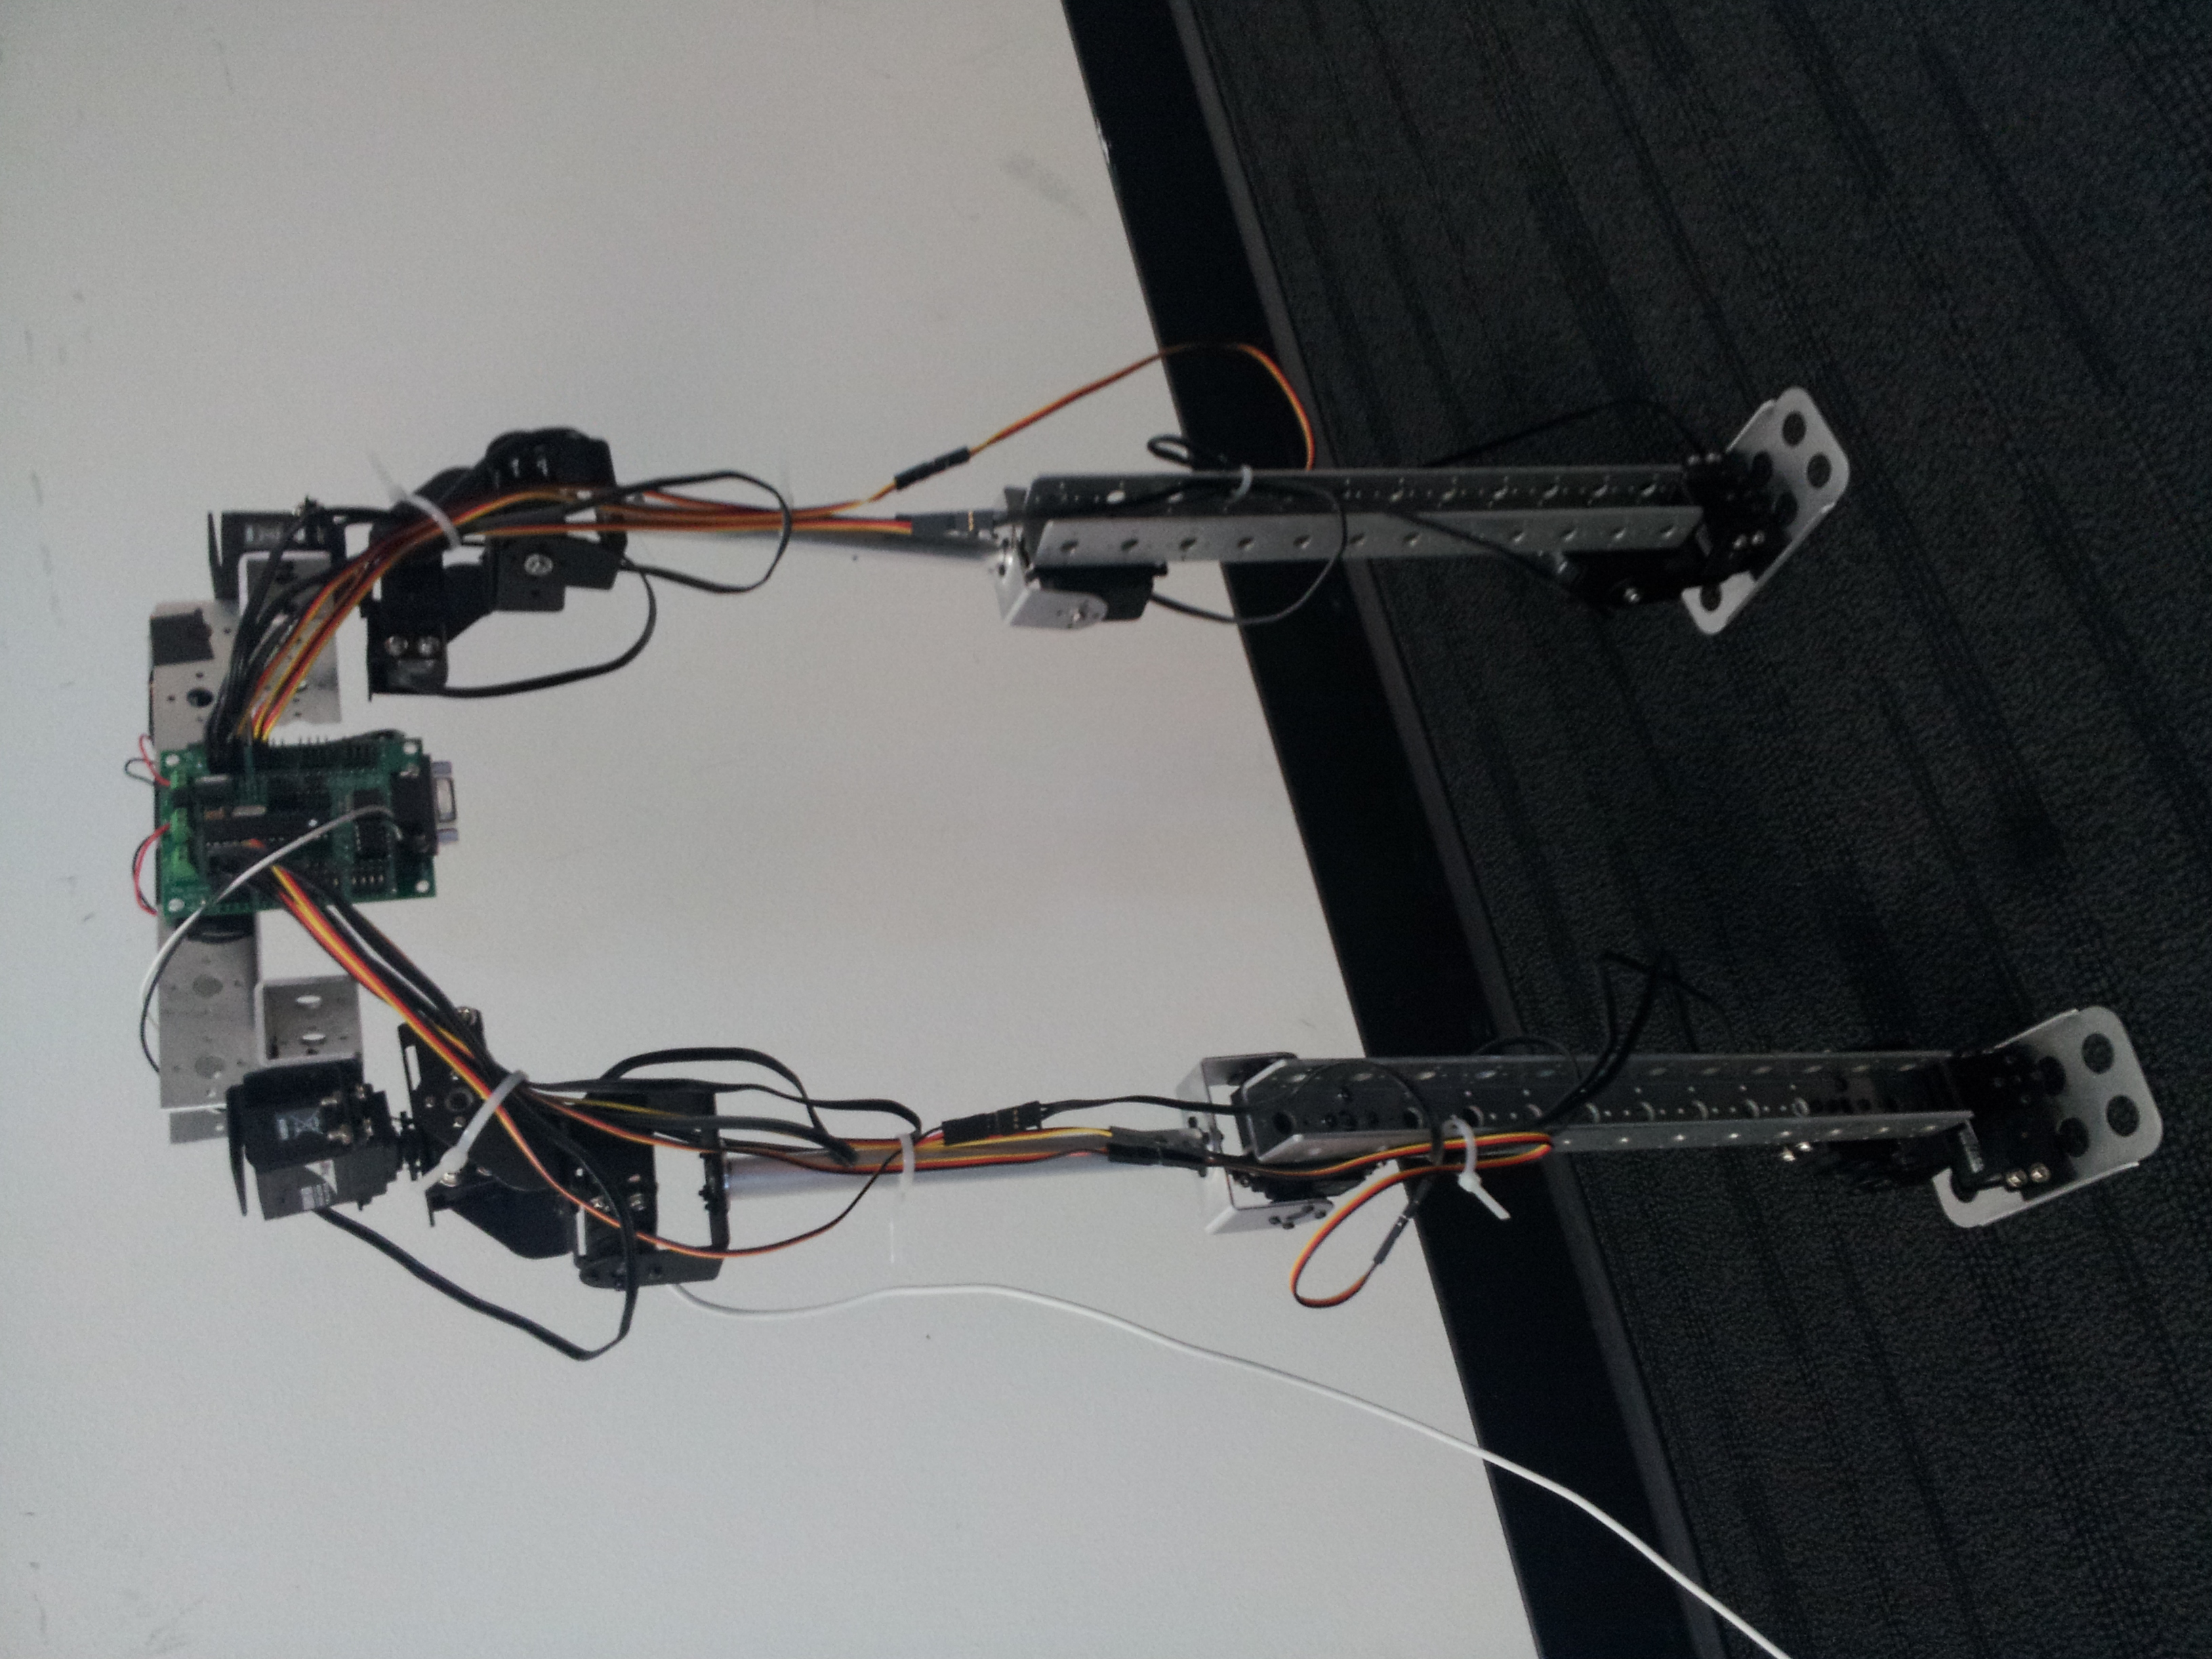
\includegraphics[width=0.7\textwidth,angle=270]{figures/LegPrototype.jpg}
  \caption{Prototype leg constructed of aluminum. Total of 6 degrees of freedom
  on each leg. The servo controller is attached to the hip}
  \label{protolegfig}
\end{figure}

\paragraph{}We performed tests on each individual servo to determine the range
of motion of each joint and the corresponding P values for the servo controller.
Figure \ref{servosetupfig} shows the configuration of the servos on the leg, as
well as their direction and range of motion in terms of SSC-32 position values.

\begin{figure}
  \centering
    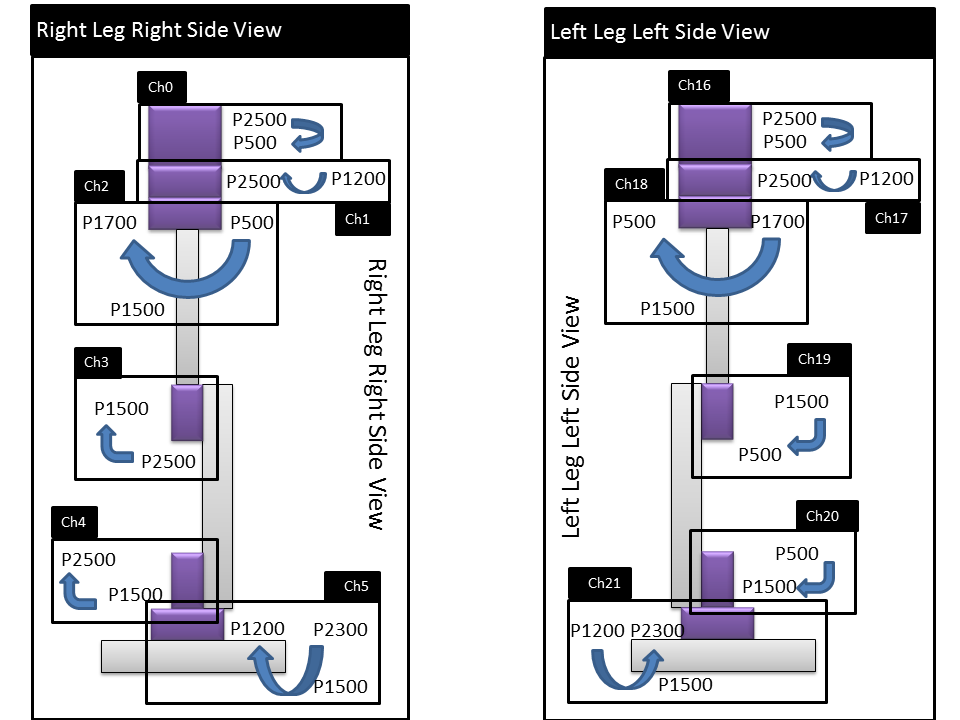
\includegraphics[width=1.0\textwidth]{figures/LegConfiguration.png}
  \caption{Location of the servos on the leg, and the directions and ranges of
  motion for each servo in terms of the SSC-32 position outputs}
  \label{servosetupfig}
\end{figure}

\subsection{Firmware}
\paragraph{}The currently completed firmware components are the serial
communications to different devices, servo control, and accelerometer control.
The communications channels implemented are the USB communications between the
PIC32 and the PC, the UART connection between the PIC32 and the SSC-32 servo
controller, and the I2C connection to the MPU6050 sensors. The I2C connection
can be adapted to more sensors that may be added in the future for other
devices. 

\paragraph{}The servo controls are accessed through \verb!SSCServo.h! which
contains functions and settings for controlling servo position through the
SSC-32 controller. The MPU6050 is accessed through \verb!MPU6050.h! which
defines memory addresses of the MPU6050 registers and functions for reading the
output of the sensors and configuring the sensor settings. Future users of the
robot can adapt these settings to program and prototype their own control
algorithms.

\subsection{Locomotion Controller}
\paragraph{}Ziqi performed the simulations of the robot leg locomotion
algorithms, and obtained the optimal parameters for equations \ref{phi3} and
\ref{phi4}. The following are the parameters we used. Refer to Ziqi's report for
a detailed analysis of the control system.
\begin{verbatim}
phi_3:           phi_4:
a13L =   73.11;  a14L =  14.91;
b13L =   19.69;  b14L = 0.8727;
c13L = -0.6449;  c14L =  4.016;
a23L =   52.58;  a24L =  1.559;
b23L =  0.6307;  b24L =   19.4;
c23L =   2.671;  c24L = -1.197;
a33L =   12.35;  a34L =  27.52;
b33L =   12.05;  b34L =  15.42;
c33L =  -2.836;  c34L = 0.9818;
a43L =   3.357;  a44L =  28.88;
b43L =   29.81;  b44L =  45.43;
c43L =  -0.797;  c44L = -5.819;
a53L =   62.63;  a54L =  15.08;
b53L =   20.15;  b54L =  31.49;
c53L =   2.236;  c54L =  1.844;
a63L =   12.04;  a64L =  1.769;
b63L =   5.405;  b64L =  9.852;
c63L =   3.598;  c64L = -5.219;
a73L =   1.786;  a74L =   31.1;
b73L =   34.76;  b74L =  45.58;
c73L =   1.995;  c74L = -2.751;
a83L =   1.418;
b83L =    47.2;
c83L =  -0.402;
\end{verbatim}

\subsection{Robot Control}
\paragraph{}The robot is controlled through a serial connection to the computer.
The PIC32MX795F512L is connected to the PC through the USB connection on UART
channel 0. Commands can be passed into the robot from a serial terminal on the
PC. Currently there are three modes of operation: Standing, Walking, and Direct
Control. Activated by sending the strings \verb!stand!, \verb!walk!, and
\verb!direct! through the serial terminal to the PIC32. While in stand mode, the
robot holds a rigid upright position. Upon completion of the balancing algorithm
begin designed by Li Yanchen, the algorithm can be implemented into the standing
mode. While in walk mode, the robot attempts to walk according to the sine waves
laid out by equations \ref{phi3} to \ref{thetaknee}. We are currently lacking a
balance algorithm, which limits the walking of the robot. In direct mode, each
servo can be commanded directly using the SSC-32 commands; in this mode all the
commands passed to the PIC32 are redirected to the SSC-32. Servos on the right
leg are attached to channels 0-5 on the SSC-32 and the servos on the left leg
are on channels 16-21. Figure \ref{servosetupfig} shows the corresponding
channels for each servo.

\subsection{Other Project Subsystems}
\subsubsection{Robot Arm}
\paragraph{}The robot arm is built using the same structure as the leg. The
shoulder consists of three servos mimicking a ball joint. The elbow is one
joint, and the wrist is two servos like the ankle. Rather than using a periodic
controller like the legs, the arm utilizes a fuzzy logic based control system.
The system takes a desired arm position and tries to manipulate the servo
positions to move the arm towards the location.

\subsubsection{Robot Hand and SMA}
\paragraph{}The robotic hand was designed in CAD by team member Helen Lopez. The
robotic hand consists of five fingers with three joints each. Each joint can be
activated and controlled through belts. The primary drive box is located in the
wrist of the robot, and the other joints are accessed through belts. 

\paragraph{}Our team could not get appreciable motion through shape memory
alloy. Electrical activation of the SMA could not be used to control the motion
we needed in the hand. More testing will need to be done to generate data for
the SMA actuation.

\section{Conclusion}
\paragraph{}Currently the robot has legs and arms that can be used as testing
platforms for various algorithms. Future groups can utilize this robotic
platform as a foundation for developing more complex control systems and
artificial intelligence software. The overall vision laid out by the our
industry adviser at the beginning of the project was of a humanoid robot that
has advanced locomotion capabilities such as running and jumping and advanced
vision and hand manipulation capabilities. The goal for our group was to build
the foundations of this robot. We have successfully prototyped the simpler
components like the leg and arm, and we have laid the software foundations for
the control system and computer vision system. It would be easy for future teams
to build on the software and hardware we have to complete the vision of our
sponsor.

\paragraph{}More testing and simulations need to be done to finish the control
systems of the robot. The control of the balance still needs to be worked on to
complete the standing and walking of our robot. More degrees of freedom can also
be added to implement more human like motions. Once that is completed more work
can be done to push it beyond the state of the art, by implementing complex
motions such as bipedal running. The vision system needs to be completed and
interfaced to the robot arm, so the vision can be used to guide the arm's
motions. We faced difficulties in the mechanical design of the hand with the
constraints of size and weight, especially in implementing SMA into the design,
so more work and testing need to be done in this area.

\paragraph{}The areas of advanced robotic locomotion, computer vision, and
advanced humanoid hand and feet design are all great areas for the sponsor Bay
Area IP to explore IP opportunities. These technologies can bring many benefits
to areas such as manufacturing and prosthetics.

\printbibliography

\end{document}
